\documentclass[12pt]{article}
\usepackage{graphicx,../lp,amsmath,url,hyperref}
%psfig
% Cross-references for handout numbers.
\usepackage{amsfonts}
%\usepackage{amsthm}
\usepackage{hyperref}
\usepackage{amssymb}
%\usepackage[capitalize]{cleveref}
\usepackage{xcolor}

%\input{handouts}

\newcounter{chapnum}

\newtheorem{definition}{Definition}[chapnum]
\newtheorem{remark}{Remark}[chapnum]
\newtheorem{theorem}{Theorem}[chapnum]
\newtheorem{lemma}[theorem]{Lemma}
\newtheorem{corollary}[theorem]{Corollary}
\newtheorem{proposition}[theorem]{Proposition}
\newtheorem{claim}[theorem]{Claim}
\newtheorem{observation}{Observation}[chapnum]

\renewcommand{\thesection}{\arabic{chapnum}.\arabic{section}}
\renewcommand{\thefigure}{\arabic{chapnum}.\arabic{figure}}


\newenvironment{proof}{\noindent{\bf Proof:} \hspace*{1em}}{
        \hspace*{\fill} $\triangle$ }
\newenvironment{proof_of}[1]{\noindent {\bf Proof of #1:}
        \hspace*{1em} }{\hspace*{\fill} $\triangle$ }
\newenvironment{proof_claim}{\begin{quotation} \noindent}{
        \hspace*{\fill} $\diamond$ \end{quotation}}
\newenvironment{solution}{\noindent{\bf Solution:} \hspace*{1em}}{
        \hspace*{\fill} $\triangle$ }


\newcommand{\R}{{\mathbb R}}
\newcommand{\Z}{{\mathbb Z}}
\newcommand{\Q}{{\mathbb Q}}
\newcommand{\C}{{\mathbb C}}
\newcommand{\N}{{\mathbb N}}
\newcommand{\lin}{\operatorname{lin}}
\newcommand{\aff}{\operatorname{aff}}
\newcommand{\cone}{\operatorname{cone}}
\newcommand{\conv}{\operatorname{conv}}
\newcommand{\vol}{\operatorname{vol}}
\newcommand{\poly}{\operatorname{poly}}




\newcommand{\CF}[1]{{\color{purple}[CF: #1]}}


\newlength{\toppush}
\setlength{\toppush}{2\headheight}
\addtolength{\toppush}{\headsep}

\newcommand{\htitle}[2]{\noindent\vspace*{-\toppush}\newline\parbox{6.5in}
{Massachusetts Institute of Technology \hfill 18.453: Combinatorial Optimization 
\newline
\textbf{Instructor:} Cole Franks \quad \textbf{Notes: }Michel Goemans and Zeb Brady \hfill#2\newline
\mbox{}\hrulefill\mbox{}}\vspace*{1ex}\mbox{}\newline
\begin{center}{\Large\bf #1}\end{center}}

\newcommand{\handout}[2]{\thispagestyle{empty}
 \markboth{ #1 \hfil #2}{ #1 \hfil #2}
 \pagestyle{myheadings}\htitle{#1}{#2}}


\setlength{\oddsidemargin}{0pt}
\setlength{\evensidemargin}{0pt}
\setlength{\textwidth}{6.5in}
\setlength{\topmargin}{0in}
\setlength{\textheight}{8.5in}


\newcounter{exercisenum}
\newcounter{exercisetot}
\setcounter{exercisetot}{0}



\newenvironment{exercises}{
	\begin{list}{{\bf Exercise \arabic{chapnum}-\arabic{exercisenum}. \hspace*{0.5em}}}
	{\setlength{\leftmargin}{0em}
	 \setlength{\rightmargin}{0em}
	 \setlength{\labelwidth}{0em}
	 \setlength{\labelsep}{0em}
	\usecounter{exercisenum}
      \setcounter{exercisenum}{\theexercisetot}}}{\setcounter{exercisetot}{\theexercisenum}\end{list}}


\newenvironment{pseudocode}{
    \begin{list}{}{
        \renewcommand{\makelabel}{$\triangleright$}
        \setlength{\topsep}{0pt}
        \setlength{\leftmargin}{32pt}
        \setlength{\labelwidth}{14pt}
        \setlength{\labelsep}{0mm}
        \setlength{\itemindent}{0mm}
        \setlength{\itemsep}{-3pt}
        \setlength{\itemsep}{0mm}
        \setlength{\parsep}{0pt}%
        \setlength{\listparindent}{0pt}
    }
}
{
    \end{list}
}


\setcounter{chapnum}{1}


\begin{document}
\handout{\arabic{chapnum}. Lecture notes on bipartite matching}{\today}
% check link for Jacobi
% check Hungarian story
% check matlab links, etc.

\bigskip

Matching problems are among the fundamental problems in combinatorial
optimization. In this set of notes, we focus on the case when the
underlying graph is bipartite.  

We start by introducing some basic graph terminology. A {\it graph}
$G=(V,E)$ consists of a set $V$ of {\it vertices} and a set $E$ of
pairs of vertices called {\it edges}. For an edge $e=(u,v)$, we say
that the {\it endpoints} of $e$ are $u$ and $v$; we also say that $e$
is {\it incident} to $u$ and $v$.  A graph $G=(V,E)$ is {\it
bipartite} if the vertex set $V$ can be partitioned into two sets $A$
and $B$ ({\it the bipartition}) such that no edge in $E$ has both
endpoints in the same set of the bipartition. A matching $M\subseteq
E$ is a collection of edges such that every vertex of $V$ is incident
to at most one edge of $M$. If a vertex $v$ has no edge of $M$
incident to it then $v$ is said to be {\it exposed} (or unmatched). A
matching is {\it perfect} if no vertex is exposed; in other words, a
matching is perfect if its cardinality is equal to $|A|=|B|$.

\begin{figure}[htbp]
\begin{center}
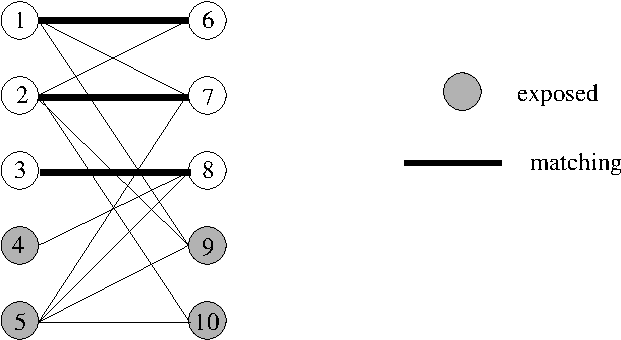
\includegraphics{../figures/bipartite}
\end{center}
\caption{Example. The edges $(1,6)$, $(2,7)$ and $(3,8)$ form a
matching. Vertices 4, 5, 9 and 10 are exposed. }
\label{bipartite}
\end{figure}

We are interested in the following two problems:

\medskip
\noindent {\bf Maximum cardinality matching problem:} Find a matching
$M$ of maximum size.

\medskip
\noindent {\bf Minimum weight perfect matching problem:} Given a cost
$c_{ij}$ for all $(i,j)\in E$, find a perfect matching of minimum cost
where the cost of a matching $M$ is given by $c(M)=\sum_{(i,j)\in M}
c_{ij}$. This problem is also called the {\it assignment problem}.

\medskip
Similar problems (but more complicated) can be defined on
non-bipartite graphs. 


\section{Maximum cardinality matching problem}

Before describing an algorithm for solving the maximum cardinality
matching problem, one would like to be able to prove optimality of a
matching (without reference to any algorithm). For this purpose, one
would like to find upper bounds on the size of any matching and hope
that the smallest of these upper bounds be equal to the size of the
largest matching. This is a {\it duality} concept that will be ubiquitous in
this subject. In this case, the dual problem will itself be a
combinatorial optimization problem. 

A {\it vertex cover} is a set $C$ of vertices such that all edges $e$
of $E$ are incident to at least one vertex of $C$. In other words,
there is no edge completely contained in $V-C$ (we use both $-$ and
$\setminus$ to denote the difference of two sets). Clearly, the size
of any matching is at most the size of any vertex cover. This follows
from the fact that, given any matching $M$, a vertex cover $C$ must
contain at least one of the endpoints of each edge in $M$. We have
just proved {\it weak duality}: The maximum size of a matching is at
most the minimum size of a vertex cover. As we'll prove later in these
notes, equality in fact holds:
\begin{theorem}[K\"onig 1931]
For any bipartite graph, the maximum size of a matching is equal to
the minimum size of a vertex cover. 
\end{theorem}

We shall prove this {\it minmax} relationship algorithmically, by
describing an efficient algorithm which simultaneously gives a maximum
matching and a minimum vertex cover. K\"onig's theorem gives a {\it
good characterization} of the problem, namely a simple proof of
optimality.  In the example above, one can prove that the matching
$(1,9)$, $(2,6)$, $(3,8)$ and $(5,7)$ is of maximum size since there
exists a vertex cover of size 4. Just take the set $\{1,2,5,8\}$.


The natural approach to solving this cardinality matching problem is
to try a {\it greedy} algorithm: Start with any matching (e.g.\ an
empty matching) and repeatedly add disjoint edges until no more edges
can be added.  This approach, however, is not guaranteed to give a
maximum matching (convince yourself).  We will now present an
algorithm that does work, and is based on the concepts of {\it
alternating paths} and {\it augmenting paths}. A path is simply a
collection of edges $(v_0,v_1), (v_1, v_2)$, $\ldots, (v_{k-1},v_k)$
where the $v_i$'s are distinct vertices. A path can simply be
represented as $v_0$-$v_1$-$\ldots$-$v_k$.

\begin{definition}
An {\bf alternating path with respect to $M$} is a path that
alternates between edges in $M$ and edges in $E - M$.
\end{definition}

\begin{definition}
An {\bf augmenting path with respect to $M$} is an alternating path
in which the first and last vertices are exposed.
\end{definition}

In the above example, the paths 4-8-3, 6-1-7-2 or 5-7-2-6-1-9 are
alternating, but only the last one is augmenting. Notice that an
augmenting path with respect to $M$ which contains $k$ edges of $M$
must also contain exactly $k+1$ edges not in $M$. Also, the two
endpoints of an augmenting path must be on different sides of the
bipartition.  The most interesting property of an augmenting path $P$
with respect to a matching $M$ is that if we set $M' = M
\bigtriangleup P \equiv (M - P)
\cup (P - M)$, then we get a matching $M'$ and, moreover, the
size of $M'$ is one unit larger than the size of $M$.  That is, we can
form a larger matching $M'$ from $M$ by taking the edges of $P$ not in
$M$ and adding them to $M'$ while removing from $M'$ the edges in $M$
that are also in the path $P$. We say that we have {\it augmented $M$
along $P$}.

The usefulness of augmenting paths is given in the following theorem.
\begin{theorem}
A matching $M$ is maximum if and only if there are no augmenting paths
with respect to $M$.
\end{theorem}

\begin{proof}(By contradiction)

($\Rightarrow$)  Let $P$ be some augmenting
path with respect to $M$.  Set $M' = M \bigtriangleup P$.  Then $M'$ is
a matching with cardinality greater than $M$.  This contradicts the
maximality of $M$.

($\Leftarrow$)  If $M$ is not maximum, let $M^*$ be a maximum matching
(so that $|M^*| > |M|$).  Let $Q = M \bigtriangleup M^*$.  Then:

\begin{itemize}
\item $Q$ has more edges from $M^*$ than from $M$ (since $|M^*| > |M|$
implies that $|M^*-M|> |M-M^*|$).

\item Each vertex is incident to at most one edge in $M \cap Q$ and
one edge $M^{*} \cap Q$.

\item Thus $Q$ is composed of cycles and paths that alternate between
edges from $M$ and $M^*$.

\item Therefore there must be some path with more edges from $M^*$ in
it than from $M$ (all cycles will be of even length and have the same
number of edges from $M^*$ and $M$).  This path is an augmenting path
with respect to $M$.
\end{itemize}

Hence there must exist an augmenting path $P$ with respect to $M$, which
is a contradiction.
\end{proof}

This theorem motivates the following algorithm.  Start with any
matching $M$, say the empty matching. Repeatedly locate an augmenting
path $P$ with respect to $M$, augment $M$ along $P$ and replace $M$ by
the resulting matching. Stop when no more augmenting path exists. By
the above theorem, we are guaranteed to have found an optimum
matching. The algorithm terminates in $\mu$ augmentations, where $\mu$
is the size of the maximum matching. Clearly, $\mu\leq \frac{n}{2}$
where $n=|V|$.

In the example, one would thus augment $M$ along an augmenting path,
say 5-7-2-6-1-9, obtain the matching $(1,9)$, $(2,6)$, $(3,8)$ and
$(5,7)$, and then realize that no more augmenting paths can be found.

The question now is how to decide the existence of an
augmenting path and how to find one, if one exists.
These tasks can be done as follows. 
Direct edges in $G$ according to $M$ as follows :
An edge goes from $A$ to $B$ if it
does not belong to the matching $M$ and from $B$ to $A$ if it does.
Call this directed graph $D$. 

\begin{claim} \label{claim:dipa}
There exists an augmenting path in $G$ with respect to $M$ iff there
exists a directed path in $D$ between an exposed vertex in $A$ and an
exposed vertex in $B$.
\end{claim}

\begin{exercises}
\item
Prove claim \ref{claim:dipa}.
\end{exercises}

This gives an $O(m)$ algorithm (where $m=|E|$) for finding an
augmenting path in $G$.  Let $A^{*}$ and $B^{*}$ be the set of exposed
vertices w.r.t. $M$ in $A$ and $B$ respectively.  We can simply attach
a vertex $s$ to all the vertices in $A^{*}$ and do a
depth-first-search from $s$ till we hit a vertex in $B^{*}$ and then
trace back our path.  


Thus the overall complexity of finding a maximum
cardinality matching is $O(nm)$.  This can be improved to
$O(\sqrt{n}m)$ by augmenting along several augmenting paths
simultaneously (for details, look up the ``Hopcroft-Karp'' algorithm).

If there is no augmenting path with respect to $M$, then we can also
use our search procedure for an augmenting path in order to construct
an optimum vertex cover. Consider the set $L$ (for Labelling) of
vertices which can be reached by a directed path from an exposed
vertex in $A$.

\begin{claim}
When the algorithm terminates, $C^*=(A-L)\cup (B\cap L)$ is a vertex
cover. Moreover, $|C^*|=|M^*|$ where $M^*$ is the matching returned by
the algorithm.
\end{claim}
This claim immediately proves K\"onig's theorem.

\begin{proof}
We first show that $C^*$ is a vertex cover. Assume not. Then there
must exist an edge $e=(a,b)\in E$ with $a\in A\cap L$ and $b\in
(B-L)$. The edge $e$ cannot belong to  the matching. If it did, then
$b$ should be in $L$ for otherwise $a$ would not be in $L$. Hence, $e$
must be in $E-M$ and is therefore directed from $A$ to $B$. This
therefore implies that $b$ can be reached from an exposed vertex in
$A$ (namely go to $a$ and then take the edge $(a,b)$), contradicting
the fact that $b\notin L$.

To show the second part of the proof, we show that $|C^*|\leq |M^*|$,
since the reverse inequality is true for any matching and any vertex
cover. The proof follows from the following observations.
\begin{enumerate} \item No vertex in $A-L$ is exposed by definition of
$L$, \item No vertex in $B\cap L$ is exposed since this would imply
the existence of an augmenting path and, thus, the algorithm would not
have terminated,
\item
There is no edge of the matching between a vertex $a\in (A-L)$ and a
vertex $b\in(B\cap L)$. Otherwise, $a$ would be in $L$.
\end{enumerate}
These remarks imply that every vertex in $C^*$ is matched and moreover
the corresponding edges of the matching are distinct. Hence,
$|C^*|\leq |M^*|$.
\end{proof}

Although the concepts of maximum matchings and minimum vertex covers
can be defined also for general (i.e.\ non-bipartite) graphs, we
should remark that K\"onig's theorem does not generalize to all
graphs. Indeed, although it is true that the size of a maximum
matching is {\it always} at most the minimum size of a vertex cover,
equality does not necessarily hold. Consider indeed the cycle $C_3$
on 3 vertices (the smallest non-bipartite graph). The maximum matching
has size 1, but the minimum vertex cover has size 2. We will derive a
minmax relation involving maximum matchings for general graphs, but it
will be more complicated than K\"onig's theorem.  

\subsection*{Exercises}
\begin{exercises}
\item 
An {\it edge cover} of a graph $G=(V,E)$ is a subset of $R$ of $E$ such that
every vertex of $V$ is incident to at least one edge in $R$.  Let $G$
be a bipartite graph with no isolated vertex.  Show that the
cardinality of the minimum edge cover $R^*$ of $G$ is equal to $|V|$
minus the cardinality of the maximum matching $M^*$ of $G$.  Give an
efficient algorithm for finding the minimum edge cover of $G$. Is this
true also for non-bipartite graphs? 

\item
Show that in any graph $G=(V,E)$ (not necessarily bipartite), the size
of {\it any maximal} matching $M$ (i.e. a matching $M$ in which one
cannot add an edge while keeping it a matching) is at least half the
size of a {\it maximum} matching $M^*$. 

%%%%%%%%%%%%%
\item Consider the problem of perfectly tiling a subset of a checkerboard
  (i.e. a collection of unit squares, see example below) with dominoes
  (a domino being 2 adjacent squares).
\begin{enumerate}
\item
Show that this problem can be formulated as the problem of deciding
whether a bipartite graph has a perfect matching. 
\item 
Can the following figure be tiled by dominoes? Give a tiling or
  a short proof that no tiling exists.

\begin{center}
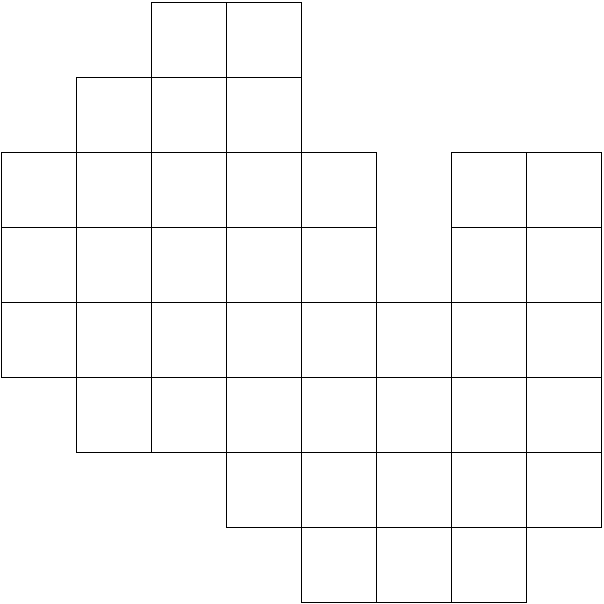
\includegraphics[height=2.5in]{../figures/domino}
\end{center}
\end{enumerate}

%%%%%%%%%%%%%%%
\item
Consider a $m\times n$ checkerboard where $m$ is even, and cells are alternatively colored black and white. Show that if we remove arbitrarily one black cell and one white cell, the resulting $mn-2$ cells can be covered by dominoes. 

%%%%%%%%%%%% 
\item
% from Korte-Vygen's book
Consider a bipartite graph $G=(V,E)$ with bipartition $(A,B)$: $V=A
\cup B$. Assume that, for some vertex sets $A_1\subseteq A$ and $B_1
\subseteq B$, there exists a matching $M_A$ covering all vertices in
$A_1$ and a matching $M_B$ covering all vertices in $B_1$. Prove that
there always exists a matching covering all vertices in $A_1\cup
B_1$.

%%%%%%%%%%%%%%%%%%
\item
Consider a bipartite graph $G=(V,E)$ with bipartition $(A,B)$
($V=A\cup B$). Let ${\cal I}=\{X\subseteq A:$ there exists a matching
$M$ of $G$ such that all vertices of $X$ are matched$\}$. 

Show that 
\begin{enumerate}
\item
If $X\in {\cal I}$ and $Y\subseteq X$ then $Y\in {\cal I}$.
\item
If $X, Y\in {\cal I}$ and $|X|<|Y|$ then there exists $y\in Y\setminus
X$ such that $X\cup\{y\}\in {\cal I}$. 
\end{enumerate}
(Later in the class, we will discuss matroids, and properties (i) and
(ii) form the definition of independent sets of a matroid.)
 
%%%%%%%%%%%%%%
\item
% Slither game, ex p.144 in Cook et al.'s book
Consider the following 2-person game on a (not necessarily bipartite)
graph $G=(V,E)$. Players 1 and 2 alternate and each selects a (yet
unchosen) edge $e$ of the graph so that $e$ together with the
previously selected edges form a simple path. The first player unable
to select such an edge loses. Show that if $G$ has a {\it perfect}
matching then player 1 has a winning strategy. 

\end{exercises}

\subsection{Hall's Theorem}

Hall's theorem gives a necessary and sufficient condition for a
bipartite graph to have a matching which saturates (or matches) all
vertices of $A$ (i.e.~a matching of size $|A|$).

\begin{theorem}[Hall 1935]
Given a bipartite graph $G=(V,E)$ with bipartition $A,B$ ($V=A\cup
B$), $G$ has a matching of size $|A|$ if and only if for every
$S\subseteq A$ we have $|N(S)|\geq |S|$, where $N(S)=\{b\in B: \exists
a \in S$ with $(a,b)\in E\}$.
\end{theorem}

Clearly, the condition given in Hall's theorem is necessary; its
sufficiency can be derived from K\"onig's theorem.

\begin{exercises}
%%%%%%%%%%%%%%%
\item
Deduce Hall's theorem from K\"onig's theorem.\\
%%%%%%%%%%
\item
Consider a bipartite graph $G=(V,E)$ with bipartition $(A,B)$. For
$X\subseteq A$, define $\operatorname{def}(X)=|X|-|N(X)|$ where $N(X)=\{b\in B:
\exists a\in X$ with $(a,b)\in E\}$. Let $$\operatorname{def}_{max}=
\max_{X\subseteq A} \operatorname{def}(X).$$ Since $\operatorname{def}(\emptyset)=0$, we have
$\operatorname{def}_{max}\geq 0$.  
\begin{enumerate}
\item
Generalize Hall's theorem by showing that the maximum size of a
matching in a bipartite graph $G$ equals $|A|-\operatorname{def}_{max}$. 
\item
For any 2 subsets $X, Y\subseteq A$, show that 
$$\operatorname{def}(X\cup Y) + \operatorname{def}(X\cap Y) \geq \operatorname{def}(X) + \operatorname{def}(Y).$$
(This can be used to show, in a different way, that the subsets from Exercise 1-7 form a matroid.)
\item (Optional:) Consider a 0-1 matrix. How are the following things related? 1. The maximal number of rooks (as in chess) that can be placed on a 1 in the matrix without attacking one another. 2. The minimal number of vertical or horizontal lines that contain all the 1's in the matrix. 3. The $a\times b$ all-zero submatrix with $a + b$ largest.
\end{enumerate}
%%%%%%%%%%%%%%
\item
Let $S=\{1,2, \cdots, n\}$. Let $A_k$ be the set of all subsets of $S$ of cardinality $k$ (thus $|A_k|={n \choose k}$). Let $k<\frac{n}{2}$. Consider the graph $G_k$ with bipartition $A_k$ and $A_{k+1}$, and with $E=\{(a,b) | a\in A_k, b\in A_{k+1}$ and $a\subset b\}$. 
\begin{enumerate}
\item
Prove that the maximum matching in $G_k$ has size $A_k$ (remember $k<n/2$). 
\item
Prove {\it Sperner's lemma}. The maximum number of subsets of $S$ such that no subset is contained into another is ${n \choose {\lfloor n/2 \rfloor}}$.  
\end{enumerate}
\end{exercises}

\section{Minimum weight perfect matching}

By assigning infinite costs to the edges not present, one can assume
that the bipartite graph is complete. The minimum cost (weight) {\it
perfect} matching problem is often described by the following story:
There are $n$ jobs to be processed on $n$ machines or computers and
one would like to process exactly one job per machine such that the
total cost of processing the jobs is minimized. Formally, we are given
costs $c_{ij}\in\R\cup\{\infty\}$ for every $i\in A, j\in B$ and the
goal is to find a perfect matching $M$ minimizing $\sum_{(i,j)\in M}
c_{ij}$.

In these notes, we present an algorithm for this problem which is
based upon linear programming, and we will take this opportunity to
illustrate several important concepts in linear programming. These
concepts will be formalized and generalized in a subsequent chapter. 

The first algorithm given for the assignment problem was given by Kuhn
[1955], but he showed only finiteness of the algorithm. A refined
version was given by Jim Munkres [1957], and showed a polynomial
running time. An algorithm is polynomial-time if its running time (the
number of basic operations to run it) is upper bounded by a polynomial
in the {\it size of the input} (i.e. the number of bits needed to
represent the input). Munkres' analysis even shows that the algorithm
is {\it strongly polynomial}, and this means that the running time is
polynomial in the {\it number of numbers} involved (i.e. does not
depend on the size of the costs $c_{ij}$). In this algorithm, the
number of operations is upper bounded by $O(n^3)$ where $n=|V|$.

The algorithm is often called the Hungarian method, as it relies on
ideas developed by Hungarians, and especially K\"onig and
Egerv\'ary. In 2006, it was discovered that the method had actually
been discovered in the 19th century by Jacobi and this was
posthumously published in 1890 in Latin, see \href{http://www.lix.polytechnique.fr/~ollivier/JACOBI/jacobiEngl.htm}{http://www.lix.polytechnique.fr/$\sim$ollivier/JACOBI/jacobiEngl.htm}.

We start by giving a formulation of the problem as an {\it integer
program}, i.e.~ an optimization problem in which the variables are
restricted to integer values and the constraints and the objective
function are linear as a function of these variables. We first need to
associate a point to every matching. For this purpose, given a
matching $M$, let its {\it incidence vector} be $x$ where $x_{ij}=1$
if $(i,j)\in M$ and 0 otherwise. One can formulate the minimum weight
perfect matching problem as follows: \lps & & & \mbox{Min} &
\sum_{i,j} c_{ij} x_{ij} \\ & \lefteqn{\mbox{subject to:}} \\ & & & &
\sum_j x_{ij} =1 & i\in A \\ & & & & \sum_i x_{ij} =1 & j\in B \\ & &
& & x_{ij}\geq 0 & i\in A, j\in B \\ & & & & x_{ij} \mbox{ integer} &
i\in A, j\in B.  \elps This is not a linear program, but a so-called
integer program.  Notice that any solution to this integer program
corresponds to a matching and therefore this is a valid formulation of
the minimum weight perfect matching problem in bipartite graphs.

Consider now the linear program $(P)$ obtained by dropping the
integrality constraints: \lps & & & \mbox{Min} & \sum_{i,j} c_{ij}
x_{ij} \\ & \lefteqn{\mbox{subject to:}} \\ (P) & & & & \sum_j x_{ij}
=1 & i\in A \\ & & & & \sum_i x_{ij} =1 & j\in B \\ & & & & x_{ij}\geq
0 & i\in A, j\in B.  \elps This is the linear programming {\it
relaxation} of the above integer program. In a linear program, the
variables can take fractional values and therefore there are many
feasible solutions to the set of constraints above which do not
correspond to matchings. But we only care about the {\it optimum}
solutions. The set of feasible solutions to the constraints in $(P)$
forms a {\it bounded polyhedron} or  {\it polytope}, and when 
we optimize a linear constraint over
a polytope, the optimum will be attained at one of the ``corners'' or
{\it extreme points} of the polytope. An extreme point $x$ of a set
$Q$ is an element $x\in Q$ which cannot be written as $\lambda y
+(1-\lambda) z$ with $0<\lambda<1$, $y, z\in Q$ with $y\neq z$.  (This
will be formalized and discussed in greater depth in the chapter on
polyhedral combinatorics.)

In general, even if all the coefficients of the constraint
matrix in a linear program are either 0 or 1, the extreme points of a linear
program are not guaranteed to have all coordinates integral (this is
of no surprise since the general integer programming problem is
NP-hard, while linear programming is polynomially solvable). As a
result, in general, there is no guarantee that the value $Z_{IP}$ of
an integer program is equal to the value $Z_{LP}$ of its LP
relaxation. However, since the integer program is {\it more}
constrained than the relaxation, we always have that $Z_{IP}\geq
Z_{LP}$, implying that $Z_{LP}$ is a lower bound on $Z_{IP}$ for a
minimization problem. Moreover, if an optimum solution to a linear
programming relaxation is integral (in our case, that would imply it
is the incidence vector of a perfect matching) then it must also be an optimum
solution to the integer program. 

\begin{exercises}
\item Prove this last claim.
\item
Give an example of an integer
program where $Z_{IP}\neq Z_{LP}$.
\end{exercises}

\bigskip
However, in the case of the perfect matching problem, the constraint
matrix has a very special form and one can show the following very
important result. Consider the polytope $P$ defined as follows.
\lps
 &     P   & =  &\{x:  &   \sum_j x_{ij} =1 & i\in A \\
  &        &   &  &   \sum_i x_{ij} =1 & j\in B \\
  &        &   &  &  x_{ij}\geq 0 & i\in A, j\in B\}.
\elps
\begin{theorem} \label{integral}
Any extreme point of $P$ is a 0-1 vector and, hence, is the 
incidence vector of a perfect matching. \end{theorem}
Because of the above theorem, the polytope $P$ is called the {\it bipartite perfect matching polytope}. To demonstrate the beauty of matchings, we shall give two completely
different proofs of this result, one purely algorithmic here and one
purely algebraic in the chapter on polyhedral theory. The algebraic
proof is related to the notion of {\it total unimodularity}.

To prove it algorithmically, we describe an algorithm for solving the
minimum weight perfect matching problem. The algorithm is
``primal-dual''. To explain what this means, we need to introduce the
notion of duality of linear programs, and let's do it in the specific
case of our bipartite matching problem. Suppose we have values $u_i$
for $i\in A$ and $v_j$ for $j\in B$ such that $u_i+v_j\leq c_{ij}$ for
all $i\in A$ and $j\in B$. Then for any perfect matching $M$, we have
that \begin{equation} \label{eq:dual} 
\sum_{(i,j)\in M} c_{ij} \geq \sum_{i\in A} u_i + \sum_{j\in B}
v_j.
\end{equation}
Thus, $\sum_{i\in A} u_i + \sum_{j\in B}
v_j$ is a {\it lower bound} on the cost of the minimum cost perfect
matching (for bipartite graphs). To get the best lower bound, we would
like to maximize this quantity, and therefore we obtain another linear
program  
\lps
  &  &  & \mbox{Max} &  \sum_{i\in A} u_i + \sum_{j\in B} v_j \\
  & \lefteqn{\mbox{subject to:}} \\
(D)    &        &   &  &  u_i+v_j\leq c_{ij} & i\in A, j\in B.
\elps
The constraints can be interpreted as $w_{ij}\geq 0$ where
$w_{ij}=c_{ij}-u_i-v_j$. 
This is a linear program, call it $(D)$.  So far, we have shown that this linear program $(D)$ provides a lower bound on the cost of any perfect matching, but we can even prove that it provides a lower bound on the value of any solution to the linear program $(P)$. Indeed consider any $x\in P$. We have
\begin{eqnarray*}
\sum_{i\in A} \sum_{j\in B} c_{ij} x_{ij} & \geq  & 
\sum_{i\in A} \sum_{j\in B} (u_i+v_j) x_{ij} \\
& = & \left(\sum_{i\in A} u_i \sum_{j\in B} x_{ij}\right) + \left( \sum_{j\in B} v_j \sum_{i\in A} x_{ij} \right) \\
& = & \sum_{i\in A} u_i + \sum_{j\in B} v_j,
\end{eqnarray*}
because of the constraints that $x$ satisfy. $(D)$ is the {\it dual} linear program in the sense of linear programming duality. Let $D$ denote the polyhedron $\{(u,v): u_i + v_j \leq c_{ij} \; \forall i \in A, j \in B\}$.


In summary, so far, we know that 
$$\left[\min_{\mbox{perfect matchings }M} \sum_{(i,j)\in M} c_{ij}
\right] \geq
\left[ \min_{x\in P} \sum_{(i,j)} c_{ij} x_{ij} \right]\geq \left[\max_{(u,v)\in D}
\sum_{i\in A} u_i + \sum_{j\in B} v_j\right].$$ 
If, for any instance, we could always find a feasible solution $u,v$ to
$(D)$ and a perfect matching $M$ such that we have equality in
(\ref{eq:dual}) (i.e. the cost of the perfect
matching is equal to the value of the dual solution) then we would
know that we have equality throughout, that the matching found 
is {\it optimum}, and that furthermore,
the incidence vector of the matching $M$ is optimum for the
linear program $(P)$. Given a solution $u,v$
to the dual, a perfect matching $M$ would satisfy equality if it contains
only edges $(i,j)$ such that $w_{ij}=c_{ij}-u_i-v_j=0$. This is what
is referred to as {\it complementary slackness}. However, for a given
$u,v$, we may not be able to find a {\it perfect} matching among the
edges with $w_{ij}=0$.   

The algorithm performs a series of iterations to obtain an appropriate
$u$ and $v$. It always maintains a
dual feasible solution and tries to find an ``almost'' primal feasible
solution $x$ satisfying complementary slackness. The fact that
complementary slackness is imposed is crucial in any primal-dual
algorithm. In fact, the most important (and elegant) algorithms in
combinatorial optimization are primal-dual. This is one of the most
important tool for designing efficient algorithms for combinatorial
optimization problems (for problems which, of course, admit such
efficient solutions).

More precisely, the algorithm works as follows. It first starts with
any dual feasible solution, say $u_i=0$ for all $i$ and $v_j=\min_i
c_{ij}$ for all $j$. In a given iteration, 
the algorithm has a dual feasible solution $(u,v)$ or say $(u,v,w)$.
Imposing complementary slackness means that we are interested in
matchings which are subgraphs of $E=\{(i,j): w_{ij}=0\}$. If $E$ has a perfect
matching then the incidence vector of that matching is a feasible
solution in $(P)$ and satisfies complementary slackness with the
current dual solution and, hence, must be optimal. To check whether
$E$ has a perfect matching, one can use the cardinality matching
algorithm developed earlier in these notes. If the maximum matching
output is not perfect then the algorithm will use information from the
optimum vertex cover $C^*$ to update the dual solution in such a way that
the value of the dual solution increases (we are maximizing in the
dual). 

Recall $L$ from the previous section output by the augmenting paths algorithm - it is the set of vertices reachable from exposed vertices in $A$ in the directed graph obtained by directing the vertices of $M$ from $B$ to $A$ and all others from $A \to B$. An optimal vertex cover $C^*$ for the bipartite graph with edges $E$ is obtained as $(A - L ) \cup (B \cap L)$. In particular, there is no
edge of $E$ between $A\cap L$ and $B-L$ (i.e. contained in the complement of $C^*$). In other words, for every
$i\in (A\cap L)$ and every $j\in (B-L)$, we have $w_{ij}>0$.  Let
$$\delta=\min_{i\in (A\cap L), j\in (B-L)} w_{ij}.$$ By the above
argument, $\delta>0$. The dual solution is updated as follows:
$$u_i=\left\{ \begin{array}{ll} u_i & i\in A-L \\ u_i + \delta & i \in
A\cap L \end{array} \right.$$ and $$v_j=\left\{ \begin{array}{ll} v_j
& i\in B-L \\ v_j - \delta & j \in B\cap L \end{array} \right.$$ One
easily check that this dual solution is feasible, in the sense that
the corresponding vector $w$ satisfies $w_{ij}\geq 0$ for all $i$ and
$j$. What is the value of the new dual solution? The difference
between the values of the new dual solution and the old dual solution
is equal to: $$ \delta (|A\cap L| -|B\cap L|) = \delta (|A \cap L| +
|A-L| - |A-L| - |B\cap L|) = \delta (|A|-|C^*|).$$ But by assumption $|C^*|<|A|$,
implying that the value of the dual solution strictly increases.

One repeats this procedure until the algorithm terminates. At that
point, we have an incidence vector of a perfect matching and also a
dual feasible solution which satisfy complementary slackness. They must
therefore be optimal and this proves the existence of an {\it
integral} optimum solution to $(P)$. Since, by carefully choosing the
cost function, one can make any extreme point be the {\it unique} optimum
solution to the linear program (this will be formally proved in the
polyhedral chapter), this shows that any extreme point is integral and
hence this proves Theorem \ref{integral}.

Of course, as some of the readers might have noticed, the proof is not
complete yet since one needs to prove that the algorithm indeed
terminates. This can be proved by noticing that at least one more
vertex of $B$ must be reachable from an exposed vertex of $A$ (and no
vertex of $B$ becomes unreachable), since an edge $e=(i,j)$ with $i\in
(A\cap L)$ and $j\in B-L$ now has $w_{ij}=0$ by our choice of $\delta$. 
This also gives an estimate of the number of iterations. In at most
$n/2$ iterations, all vertices of $B$ are reachable or the matching
found has increased by at least one unit. Therefore, after $O(n^2)$
iterations, the matching found is perfect. The overall running time of
the algorithm is thus $O(n^4)$ since it takes $O(n^2)$ to compute the
set $L$ in each iteration. By looking more closely at how vertices get
labelled between two increases of the size of the matching, one can
reduce the running time analysis to $O(n^3)$.

\begin{exercises}
\item
Check that the running time of the algorithm
is indeed $O(n^3)$.
\end{exercises}

\noindent {\bf Example:} Consider the instance given by the following
cost matrix defined on a bipartite graph with 5 vertices on each side
of the bipartition: 

\begin{center}
\begin{tabular}{|c|c|c|c|c|} \hline
0 & 2 & 7 & 2 & 3 \\ \hline
1 & 3 & 9 & 3 & 3 \\ \hline
1 & 3 & 3 & 1 & 2 \\ \hline
4 & 0 & 1 & 0 & 2 \\ \hline
0 & 0 & 3 & 0 & 0 \\ \hline
\end{tabular}\end{center}

Assume that $u^T=(2, 3, 0, -2, 0)$ and $v^T=(-2, 0, 3, 0, 0)$. The set $E$
of edges with $w_{ij}=0$ corresponds exactly to the set of edges in
Figure \ref{bipartite}. The maximum cardinality matching algorithm
finds the matching $(1,9)$, $(2,6)$, $(3,8)$ and $(5,7)$, and the set
of labelled vertices is $\{3,4,8\}$. We compute $\delta$ as 
$$ \delta= \min_{i\in\{3,4\}, j\in\{6,7,9,10\}} w_{ij} = 1$$
corresponding to the edge $(3,9)$. The new vectors $u$ and $v$ are
$u^T=(2, 3, 1, -1,0)$ and $v^T=(-2,0,2,0,0)$. The value of the dual
solution has increased from 4 units to 5. The corresponding set
$E$ now has a perfect matching, namely $(1,6)$, $(2,7)$, $(3,9)$,
$(4,8)$ and $(5,10)$ of cost 5. Both the matching and the dual
solution are optimal. 

\subsection*{Exercises}
\begin{exercises}
\item \label{bm:bip-reg}
Consider a bipartite graph $G=(V,E)$ in which every vertex has degree
$k$ (a so-called $k$-regular bipartite graph). Prove that such a graph
always has a perfect matching in two different ways:
\begin{enumerate}
\item
by using K\"onig's theorem,
\item
by using the linear programming formulation we have derived in this
section. 
\end{enumerate}

(Optional: Is this result also true for non-bipartite graphs?)
%%%%%%%%%%%%%%%%%%%
\item
Using the previous exercise \ref{bm:bip-reg}, show that the edges of a
$k$-regular bipartite graph $G$ can be partitioned into $k$ matchings
(i.e.~the number of colors needed to color the edges of a $k$-regular
bipartite graph such that no two edges with a common  endpoint  have
the same color --- {\it the edge chromatic number} --- is precisely $k$).


(Optional: Is this result also
true also for non-bipartite graphs?)
%%%%%%%%%%%%%%%%%%%%%%%%
\item
Given a graph $G=(V,E)$, its edge coloring number is the smallest
number of colors needed to color the edges in $E$ so that any two
edges having a common endpoint have a different color. 
\begin{enumerate}
\item
Show that the edge coloring number of a {\it bipartite} graph $G$ is
always equal to its maximum degree $\Delta$ (i.e.~the maximum over all
vertices $v$ of the number of edges incident to $v$). (Use the
previous problem.) 
\item
Give an example of a non-bipartite graph for which the edge coloring
number is (strictly) greater than $\Delta$. 
\end{enumerate}


%%%%%%%%%%%%%%%%%%
\item 
We have shown that there always exists a solution $x$ to the linear
program (P) with all components integral. Reprove this result in the
following way. 

Take a (possibly non-integral) {\it optimum} solution $x^*$. If there
are many optimum solutions, take one with as few non-integral values
$x^*_{ij}$ as possible. Show that, if $x^*$ is not integral, there
exists a cycle $C$ with all edges $e=(i,j)\in C$ having a non-integral
value $x^*_{ij}$. Now show how to derive another optimum solution with
fewer non-integral values, leading to a contradiction.\\

(Optional:) Conclude that the doubly stochastic matrices (the set of $n\times n$ nonnegative matrices with unit row and column sums) are the convex hull of the permutation matrices (the matrices with exactly $n$ ones, no two in the same row or column).
\item
In this exercise, you will do a little experiment with the (minimum
cost) assignment problem. Take a complete bipartite graph with $n$
vertices on each side of the bipartition, and let us assume that all
$c_{ij}$ (for $i,j\in\{1,\cdots,n\}$) are all independent uniform
random variables between 0 and 1. Take 5 different values for $n$ (the
largest being a few hundreds) and for each compute the {\it minimum}
cost assignment value for 5 instances. Any guess on how this value
increases as $n$ goes to infinity. Does it seem to converge? To what
value? Surprised? (Yes, you should be, and it is normal that you do
not understand why.)

To solve the assignment problem, you can use MATLAB (it is available on
athena, or available to MIT students for download). 
To access MATLAB on athena, you need to type:

\begin{verbatim}
>> add matlab
>> matlab
\end{verbatim}

If you have never used MATLAB before, you can find some tutorial on
the \href{http://web.mit.edu/18.06/www/}{18.06 webpage}. There is a
MATLAB m-file at \href{http://www-math.mit.edu/~goemans/bghungar.m}{http://www-math.mit.edu/$\sim$goemans/bghungar.m}
which implements the Hungarian method (just put it in the directory
from which you run MATLAB). If $C$ is an $n\times n$
matrix, then 

\begin{verbatim}
>> a=bghungar(C)
\end{verbatim}

gives a vector a such that $(1,a(1)), (2,a(2)), \cdots$ is the {\it
  maximizing} matching. So to get the value of the {\it minimum}
  assignment, you can just do:

\begin{verbatim}
>> a=bghungar(-C);
>> v=sum(diag(C(1:n,a(1:n))))
\end{verbatim}

%%%%%%%%%%%%%%%%%%
\item 
%  Reingold Tarjan '81 SICOMP
  For the assignment problem, the greedy algorithm (which repeatedly
  finds the minimum cost edge disjoint from all the previously
  selected edges) can lead to a solution whose cost divided by the
  optimum cost can be arbitrarily large (even for graphs with 2
  vertices on each side of the bipartition).

Suppose now that the cost comes from a  metric, even just a line
metric. More precisely, suppose that the bipartition is $A \cup B$
with $|A|=|B|=n$ and the $i$th vertex of $A$ (resp. the $j$th vertex
of $B$) is associated with $a_i\in \R$ (resp. $b_j\in B$). Suppose
that the cost between these vertices is given by $c_{ij}=|a_i-b_j|$. 

Consider the greedy algorithm: select the closest pair of vertices,
one from $A$ and from $B$, match them together, delete them, and
repeat until all vertices are matched. For these line metric
instances, is the cost of the greedy solution always upper bounded by
a constant (independent of $n$) times the optimum cost of the
assignment? If so, prove it; if not, give a family of examples
(parametrized by $n$) such that the corresponding ratio becomes
arbitrarily large.


\end{exercises}

\end{document}
